\en

\section{Participant Observation Experiment}

For our participant observation, we attempted to mitigate two code 
duplications found by the ArKanjo tool in the AMD Display driver by applying 
our systematic approach presented in \ref{subsubsec:systematic}. 
As presented in section \ref{sec:meteth},
we opted to apply the systematic approach in the mitigations.

Table \ref{tab:patch} summarizes the impact of the mitigations in terms of 
files and lines changed and the refactoring method used. In the next sections, 
we present our experience and learning for each mitigation.

\begin{table}
\begin{tabular}{ | c | c | c | c | m{6em} | }

\hline

\textbf{Mitigation} & \textbf{Files changed} & \textbf{Lines added} & \textbf{Lines removed} & \textbf{Refactoring methods used}
\\ \hline 

1 & 13 & +224 & -753 & Parameterize Method, Extract Method  \\ \hline
2 & 8 & +132 & -517 & None \\ \hline

\hline
\end{tabular}
\caption{Early results on mitigating code duplications on the AMD Display driver.}
\label{tab:patch}
\end{table}


\subsection{Mitigation 1}

In the systematic approach, we found that the \textit{offset\_to\_id} function
exists in 10 code files, enclosing multiple GPU architectures. The duplicated
functions are not exactly equal, as some minimal specific logic is applied to 
each GPU architecture. To address this issue, we used the extract method to
break the function into smaller parts and the parameterized method to address
the specific logic for the GPUs.

We reached a point where we had a scratch on how to mitigate the duplications found, 
but we could not complete the refactoring to a state capable of submitting as a 
patch to the driver. We found that the configuration files on the AMD Display 
driver are designed to be imported at compilation time using \textit{\#define} macros. 
The configuration files' design choice makes refactoring duplications on generic 
approaches trickier, as refactoring code that depends on these files requires 
significant refactoring of the configuration files' design and deep knowledge 
of the codebase, which we, as first-time contributors, do not have. Thus, we opted 
not to continue investigating this mitigation.


\subsection{Mitigation 2}

Using the systematic approach, we found that the \textit{phy\_id\_to\_atom} function 
exists in five code files, and two other functions are duplicated
in those five code files. All functions across the files were exactly equal,
so there was no need to apply the refactoring methods presented in the literature.
The refactoring was resumed to create a generic library and fix the compilation targets.

The code files in the second mitigation do not depend on configuration files. Thus,
we did not face the same issues during the first mitigation. Refactoring the code
to mitigate duplications reached a point we judged was good enough to submit as a
patch to contribute to the AMD Display driver code quality. Thus, we moved to send
the refactoring to the driver maintainers as a patch, documenting our findings and experiences
on the process.

\begin{figure}
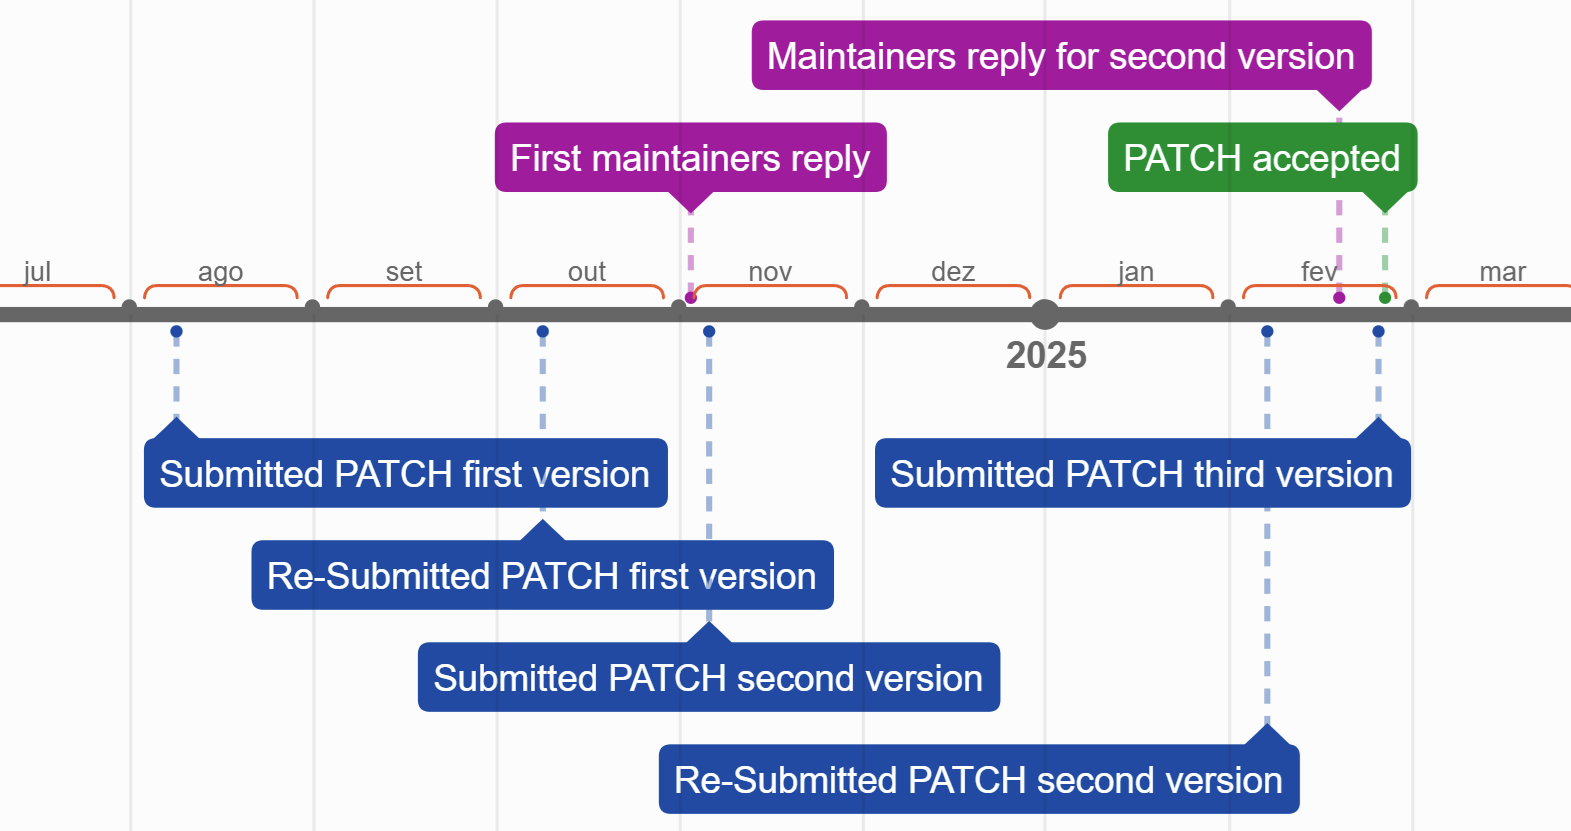
\includegraphics[scale=0.45]{timeline_patch}
\caption{Timeline of the PATCH submission process}
\label{fig:timeline}
\end{figure}

The experience of submitting a patch was not as we expected. The process took 7 
months and 16 days, significantly slower than expected. We initially submitted 
the patch on August 9, 2024, but we did not receive replies. Thus, we had to 
resend it on October 9, 2024. We received an initial response on November 3, 2024, 
requesting minimal changes. We submitted a second version with the requested 
changes on November 16, 2024. We did not receive replies initially and will 
need to resend the patch on February 7, 2025. We received a reply on 
February 11, 2025, asking for additional changes. We sent a third version on 
February 24, 2025, and the patch was accepted and integrated into the kernel 
codebase on February 25, 2025. Figure \ref{fig:timeline} illustrates the 
timeline of the patch submission.

After the initial reply from the maintainers, we observed that the review process 
became more responsive. We hypothesize that once a patch receives initial attention, 
it is more closely tracked by maintainers. Another contributing factor to the initial 
delay could be the maintainers' workload at the time of the first submission.

We discussed the Display driver with our point of contact at AMD to understand the 
reason for the slow patch submission process. We learned that some of the code in 
the driver is shared across all operating systems that support the implemented GPUs. 
This fact creates a complex process within AMD to format and submit changes across 
the supported systems while simultaneously implementing measures to mitigate errors. 
Additionally, we comprehended that AMD Display driver developers can not view 
duplicated code negatively, as we understand it is a good practice in software engineering. 
One example shared with us is that duplicated code enhances the independence of 
GPU driver code, allowing developers to make changes to a specific GPU without 
needing to test compatibility with others. This approach helps save a 
significant amount of time and effort.

Regarding the patch changes requested for the second version, the maintainers 
only asked for minor changes to align with code style, correct license use, 
and best practices that were initially unknown. For the change requested on 
the third version, the maintainers asked us to move the functions created in 
the generic library to an existing file instead of creating a new one.
\footnote{Patch submitted: \href{https://lore.kernel.org/all/20250225015532.303032-1-luanicaro@usp.br/}{lore.kernel.org/all/20250225015532.303032-1-luanicaro@usp.br}}.

The initial plan of this research was to approach and send many mitigations to collect 
many artifacts from the driver community. Still, the slow process of sending a patch 
makes this plan unviable. Thus, we opted to redirect this research to work with students 
and refactoring duplicated function pairs found by the tool directly in the IIO subsystem and the 
AMD Display driver without passing through the whole process of the systematic approach 
proposed. This alternative allowed us to collect artifacts from the students' experiences 
and findings and not be too dependent on the interaction with the kernel community. 
Another advantage is accelerating the interaction with the kernel community because we are 
not applying the systematic approach, which translates to more minor code changes.
